\documentclass[epsf]{article}
\usepackage{amsmath,amsthm,amsfonts,latexsym,amscd, framed}
\usepackage{graphicx}
%\title{Project \#2: The Accumulation Function}
%\date{Solutions due Friday, October 12th}

\textwidth=6.0truein\hoffset=-.5truein
\textheight=8.5truein\voffset=-.5truein

\begin{document}
%\maketitle
\newcommand{\R}{\mathbb{R}}
\newcommand{\noi}{\noindent}
\newcommand{\bs}{\bigskip}

%%%%


\begin{center}
{\Large Project \#1: Undoing the Chain Rule\\
\vskip 2mm
Guide for TAs}
\end{center}


\noi {\bf 1. }Get things started by either pairing students up or asking them to get with a partner.  Social awkwardness can often slow the pairing-up down, so don't be afraid to say ``you two, work together'' etc. -- more often than not, they'll be grateful for the nudge.\\

\vskip 2mm
\noi{\bf 2. } Then ask them to work on PW 1 parts (a) and (b).  Give them 2-5 minutes to get comfortable with their partners and talk about what it might mean for a function to be defined implicitly by that equation.  As them to write down an example of a function that is defined implicitly by the circle equation.  This will be an easier question to answer and it will open up for discussion about what that might mean.\\

\noi{\bf PW 1}  Recall that the circle of radius $2$ centered at $(1,3)$
is described in the plane by the equation
$(x-1)^2+(y-3)^2=4.$
\begin{itemize}
\item[(a)]  This equation does {\bf not} define a function.  Why?

\item[(b)]  However, the equation for a circle can be used to define several functions {\em implicitly}.  What do you think this means?
\end{itemize}

\noi{\bf 3.} After 2-5 minutes to think about (a) and (b) bring the whole class together.  Ask them to tell you what example ``implicitly defined'' functions they came up with.  \textit{Write three examples on the board as they tell them to you}.  
\begin{itemize}
\item Ask them why they chose the function they chose.  They will likely say something like ``the $x$ and $y$ values lie on the circle'' or something like that.  You can use whatever they say as a starting point for a reasonable definition of \textit{implicitly defined function} - which you can write on the board.  
\item Ask the class if they agree or disagree with the examples or with the definition you wrote.  This question - agree or disagree? - often draws out good questions/comments.
\item Don't be afraid to give them wait time to think - it takes them time to put ideas together.
\end{itemize}
\vskip 2mm

\noi{\bf 4.} Now instruct them to work on part (c).  Many of them will have forgotten how to get started on this one, so you may want to remind them that we think of $y$ as a function of $x$ and use the chain rule to differentiate.  You should also circulate while they work and nudge groups along if they need it.  Again, don't be afraid to leave a group while they're still thinking - it's all part of wait time.  Give them 5 minutes or so on this one.

\vskip 2mm

\begin{itemize}

\item[(c)] Use the chain rule to find the slope of a tangent line at a fixed point $(x_0, y_0)$ of the graph of
one of these implicit functions.  \\
\end{itemize}

\noi{\bf 5.} After 5 minutes or so of thinking/working on part (c), bring the group together and have them walk you through the problem at the board.  You can write the equation down and ask the students to prompt you through it.  i.e. ``What do I do first?''  ``What next?'' etc.

\vskip 2mm
\newpage

\noi{\bf 6.} After you finish up part (c), tell them to work on PW 2 parts (a) and (b).  Circulate while they work and give them 5 minutes or so to work.  If you see a fast group finish early, you can ask them to write their solution on the board to share with the class.  

\vskip 2mm

\noi{\bf PW 2} The graph of the equation $y^2=x^3-x$ is a famous elliptic curve related to the proof of Fermat's Last Theorem\footnote{see http://en.wikipedia.org/wiki/Fermat}. 

\begin{itemize}
\item[(a)] Give a formula for the slope of a tangent line to any point $(x_0, y_0)$ of this curve.  Where are the tangents vertical?

\item[(b)] Suppose a function $f(x)$ is implicitly defined by the curve $y^2=x^3-x$.  What differential equation
does $f(x)$ satisfy?  You must use the chain rule again.
\end{itemize}

\noi{\bf 7. }Now bring the class together.  Either have a group share what they got for part (a) on the board or have the class walk you through it.  Ask them, ``Do you agree or disagree?''  Once they're steered straight, have them start on the slope field.  They will likely need some explanation of what the slope field is since we will not have spent much time on this in class.  You could prompt them to make the table with $x$, $y$ and $y'$ columns and look for patterns to make their work easier.   You may want to get it started and have them finish up in their groups.
\vskip 2mm
\noi{\bf 8.} Have them think about (d) once they finish their slope fields.  i.e. if you see a group that looks done, prompt them to think about (d).

\begin{itemize}
\item[(c)] Sketch the slope-field for the differential equation in (b). Plot the elliptic curve
$y^2=x^3-x$ on the same plane.  You can use the grid on the back of this page for your slope field.

\item[(d)] Does the differential equation you came up with in part (b) have any solutions that aren't defined implicitly by the curve $y^2=x^3-x$?  If so, sketch one of these solutions on your slope-field.  If not, explain.
\end{itemize}

\noi{\bf 9.} Now model sketching this slope field for them.  Make the table and ask them if they found any helpful patterns.  If they did, \textit{write the ideas on the board}.  Go slow and be open for questions, slope fields can be a big mental jump.

\vskip 2mm

\noi{\bf 10.} Now ask the class what they think about part (d).  Can anyone sketch another curve that satisfies the DE?  If so, have them come up to the board and sketch it.  Can anyone think of an equation for another curve/function that satisfies the same DE?  If so, write that equation/function down and ask that student to explain how they can tell.  Ask the class if they agree or disagree with the examples.  
\vskip 2mm
\noi{\bf 11.} Once you've gone through the Pre-work problems, hand out the solutions pages and instruct them to commit to a partner for next week.  It's okay if they switch partners and let them know that the solutions pages are on GS if they need another copy.  Tell them solutions are due at the beginning of section next week.


\newpage


Use the dot grid below to sketch your slope field for PW 2 (c).  Sketch a dash at each $(x,y)$ gridpoint whose slope matches the value of $y'$ for the corresponding values of $(x,y)$. \\

You may find it helpful to make a table of $x$, $y$ and $y'$ values and take advantage of any symmetry you notice.
\vskip 1 in
\begin{center}
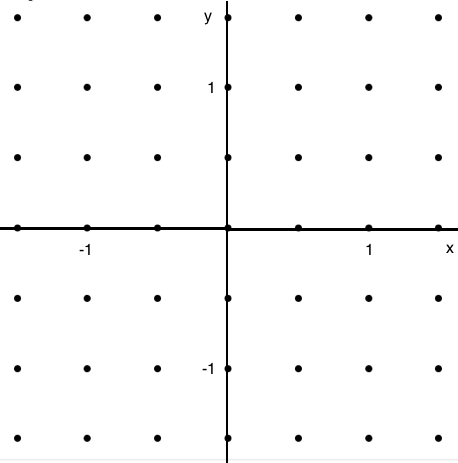
\includegraphics[width=100mm]{dotgrid.png}
\end{center}

\end{document}